% ============================================================
% Question Bank: ch03-09 Introduction to Square Roots
% Topic Title: Introduction to Square Roots
% Supplementary Topic
% Questions: 27 (15 MC + 6 SA + 6 Graphical)
% ============================================================

% --- Multiple Choice Questions (15) ---

\begin{practiceQuestion}{3-9-q01}{mc}
\begin{questionText}
What is $\sqrt{64}$?
\end{questionText}
\choiceA{$6$}
\choiceB{$7$}
\choiceC{$8$}
\choiceD{$32$}
\correctAnswer{C}
\explanation{$8 \times 8 = 64$, so $\sqrt{64} = 8$.}
\end{practiceQuestion}

\begin{practiceQuestion}{3-9-q02}{mc}
\begin{questionText}
Which number is a perfect square?
\end{questionText}
\choiceA{$18$}
\choiceB{$24$}
\choiceC{$36$}
\choiceD{$50$}
\correctAnswer{C}
\explanation{$36 = 6 \times 6$. A perfect square is the product of an integer multiplied by itself.}
\end{practiceQuestion}

\begin{practiceQuestion}{3-9-q03}{mc}
\begin{questionText}
A square garden has an area of $121$ square feet. What is the length of one side?
\end{questionText}
\choiceA{$10$ feet}
\choiceB{$11$ feet}
\choiceC{$12$ feet}
\choiceD{$13$ feet}
\correctAnswer{B}
\explanation{Side $= \sqrt{121} = 11$ feet. Because $11 \times 11 = 121$.}
\end{practiceQuestion}

\begin{practiceQuestion}{3-9-q04}{mc}
\begin{questionText}
Between which two consecutive whole numbers does $\sqrt{50}$ lie?
\end{questionText}
\choiceA{$5$ and $6$}
\choiceB{$6$ and $7$}
\choiceC{$7$ and $8$}
\choiceD{$8$ and $9$}
\correctAnswer{C}
\explanation{$7^2 = 49$ and $8^2 = 64$. Since $49 < 50 < 64$, $\sqrt{50}$ lies between $7$ and $8$.}
\end{practiceQuestion}

\begin{practiceQuestion}{3-9-q05}{mc}
\begin{questionText}
What is $\sqrt{144}$?
\end{questionText}
\choiceA{$11$}
\choiceB{$12$}
\choiceC{$13$}
\choiceD{$14$}
\correctAnswer{B}
\explanation{$12 \times 12 = 144$, so $\sqrt{144} = 12$.}
\end{practiceQuestion}

\begin{practiceQuestion}{3-9-q06}{mc}
\begin{questionText}
Which statement is true?
\end{questionText}
\choiceA{$\sqrt{25} = 5.5$}
\choiceB{$\sqrt{49} = 6$}
\choiceC{$\sqrt{81} = 9$}
\choiceD{$\sqrt{100} = 50$}
\correctAnswer{C}
\explanation{$\sqrt{81} = 9$ because $9 \times 9 = 81$. A: $\sqrt{25} = 5$. B: $\sqrt{49} = 7$. D: $\sqrt{100} = 10$.}
\end{practiceQuestion}

\begin{practiceQuestion}{3-9-q07}{mc}
\begin{questionText}
Which is the best estimate for $\sqrt{30}$?
\end{questionText}
\choiceA{$5.1$}
\choiceB{$5.5$}
\choiceC{$5.8$}
\choiceD{$6.0$}
\correctAnswer{B}
\explanation{$5^2 = 25$ and $6^2 = 36$. $30$ is about halfway, so $\sqrt{30} \approx 5.48$, closest to $5.5$.}
\end{practiceQuestion}

\begin{practiceQuestion}{3-9-q08}{mc}
\begin{questionText}
What is $\sqrt{1}$?
\end{questionText}
\choiceA{$0$}
\choiceB{$1$}
\choiceC{$-1$}
\choiceD{$2$}
\correctAnswer{B}
\explanation{$1 \times 1 = 1$, so $\sqrt{1} = 1$.}
\end{practiceQuestion}

\begin{practiceQuestion}{3-9-q09}{mc}
\begin{questionText}
A square tile has a side length of $9$ cm. What is its area?
\end{questionText}
\choiceA{$18$ cm$^2$}
\choiceB{$36$ cm$^2$}
\choiceC{$72$ cm$^2$}
\choiceD{$81$ cm$^2$}
\correctAnswer{D}
\explanation{Area $= 9^2 = 9 \times 9 = 81$ cm$^2$.}
\end{practiceQuestion}

\begin{practiceQuestion}{3-9-q10}{mc}
\begin{questionText}
Which expression equals $7$?
\end{questionText}
\choiceA{$\sqrt{14}$}
\choiceB{$\sqrt{49}$}
\choiceC{$\sqrt{77}$}
\choiceD{$\sqrt{7}$}
\correctAnswer{B}
\explanation{$\sqrt{49} = 7$ because $7 \times 7 = 49$.}
\end{practiceQuestion}

\begin{practiceQuestion}{3-9-q11}{mc}
\begin{questionText}
Between which two consecutive integers does $\sqrt{90}$ lie?
\end{questionText}
\choiceA{$8$ and $9$}
\choiceB{$9$ and $10$}
\choiceC{$10$ and $11$}
\choiceD{$44$ and $46$}
\correctAnswer{B}
\explanation{$9^2 = 81$ and $10^2 = 100$. Since $81 < 90 < 100$, $\sqrt{90}$ is between $9$ and $10$.}
\end{practiceQuestion}

\begin{practiceQuestion}{3-9-q12}{mc}
\begin{questionText}
What is $\sqrt{0}$?
\end{questionText}
\choiceA{undefined}
\choiceB{$1$}
\choiceC{$0$}
\choiceD{No real answer}
\correctAnswer{C}
\explanation{$0 \times 0 = 0$, so $\sqrt{0} = 0$.}
\end{practiceQuestion}

\begin{practiceQuestion}{3-9-q13}{mc}
\begin{questionText}
Which number is NOT a perfect square?
\end{questionText}
\choiceA{$16$}
\choiceB{$25$}
\choiceC{$40$}
\choiceD{$64$}
\correctAnswer{C}
\explanation{$16 = 4^2$, $25 = 5^2$, $64 = 8^2$. But $40$ is not a perfect square ($6^2 = 36$, $7^2 = 49$).}
\end{practiceQuestion}

\begin{practiceQuestion}{3-9-q14}{mc}
\begin{questionText}
A square room has an area of $196$ square feet. What is the perimeter?
\end{questionText}
\choiceA{$14$ feet}
\choiceB{$28$ feet}
\choiceC{$49$ feet}
\choiceD{$56$ feet}
\correctAnswer{D}
\explanation{Side $= \sqrt{196} = 14$ feet. Perimeter $= 4 \times 14 = 56$ feet.}
\end{practiceQuestion}

\begin{practiceQuestion}{3-9-q15}{mc}
\begin{questionText}
Which list shows perfect squares in order?
\end{questionText}
\choiceA{$1, 2, 4, 8, 16$}
\choiceB{$1, 4, 9, 16, 25$}
\choiceC{$2, 4, 6, 8, 10$}
\choiceD{$1, 3, 5, 7, 9$}
\correctAnswer{B}
\explanation{$1^2 = 1$, $2^2 = 4$, $3^2 = 9$, $4^2 = 16$, $5^2 = 25$. These are the first five perfect squares.}
\end{practiceQuestion}

% --- Short Answer Questions (6) ---

\begin{practiceQuestion}{3-9-q16}{sa}
\begin{questionText}
What is $\sqrt{225}$?
\end{questionText}
\correctAnswer{$15$}
\explanation{$15 \times 15 = 225$, so $\sqrt{225} = 15$.}
\end{practiceQuestion}

\begin{practiceQuestion}{3-9-q17}{sa}
\begin{questionText}
Estimate $\sqrt{72}$ to the nearest whole number.
\end{questionText}
\correctAnswer{$8$}
\explanation{$8^2 = 64$ and $9^2 = 81$. Since $72 - 64 = 8$ and $81 - 72 = 9$, $72$ is closer to $64$, so $\sqrt{72} \approx 8.49$ and rounds to $8$.}
\end{practiceQuestion}

\begin{practiceQuestion}{3-9-q18}{sa}
\begin{questionText}
A fence encloses a square yard of $400$ square meters. How long is each side?
\end{questionText}
\correctAnswer{$20$ meters}
\explanation{$\sqrt{400} = 20$ meters. $20 \times 20 = 400$.}
\end{practiceQuestion}

\begin{practiceQuestion}{3-9-q19}{sa}
\begin{questionText}
Is $\sqrt{150}$ rational or irrational? Explain.
\end{questionText}
\correctAnswer{Irrational}
\explanation{$150$ is not a perfect square ($12^2 = 144$, $13^2 = 169$), so $\sqrt{150}$ cannot be expressed as a fraction; it is irrational.}
\end{practiceQuestion}

\begin{practiceQuestion}{3-9-q20}{sa}
\begin{questionText}
What is $\sqrt{169}$?
\end{questionText}
\correctAnswer{$13$}
\explanation{$13 \times 13 = 169$, so $\sqrt{169} = 13$.}
\end{practiceQuestion}

\begin{practiceQuestion}{3-9-q21}{sa}
\begin{questionText}
Find two consecutive integers such that $\sqrt{110}$ lies between them.
\end{questionText}
\correctAnswer{$10$ and $11$}
\explanation{$10^2 = 100$ and $11^2 = 121$. Since $100 < 110 < 121$, $\sqrt{110}$ is between $10$ and $11$.}
\end{practiceQuestion}

% --- Graphical Questions (3 GMC + 3 GSA) ---

\begin{practiceQuestion}{3-9-q22}{gmc}
\begin{questionText}
The number line shows the location of $\sqrt{20}$. Between which two integers is $\sqrt{20}$ placed?

\begin{center}
\begin{tikzpicture}
  \draw[thick,->] (0,0) -- (8,0);
  \foreach \x in {0,...,7} \draw (\x,0.1) -- (\x,-0.1) node[below,font=\small] {$\x$};
  \fill[funBlue] (4.47,0) circle (0.1) node[above=4pt,font=\small] {$\sqrt{20}$};
\end{tikzpicture}
\end{center}
\end{questionText}
\choiceA{$3$ and $4$}
\choiceB{$4$ and $5$}
\choiceC{$5$ and $6$}
\choiceD{$9$ and $10$}
\correctAnswer{B}
\explanation{$4^2 = 16$ and $5^2 = 25$. Since $16 < 20 < 25$, $\sqrt{20}$ is between $4$ and $5$.}
\end{practiceQuestion}

\begin{practiceQuestion}{3-9-q23}{gmc}
\begin{questionText}
The diagram shows a square with area $A$. What is the side length?

\begin{center}
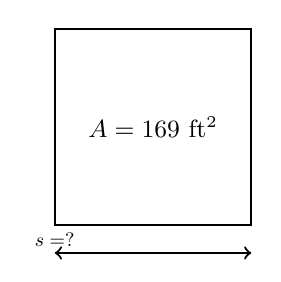
\begin{tikzpicture}[scale=0.78]
  \draw[thick] (0,0) rectangle (3.2,3.2);
  \node[font=\small] at (1.6,1.6) {$A = 169$ ft$^2$};
  \draw[thick,<->] (0,-0.45) -- (3.2,-0.45);
  \node[midway,below,font=\small] at (1.6,-0.45) {$s = ?$};
\end{tikzpicture}
\end{center}
\end{questionText}
\choiceA{$11$ ft}
\choiceB{$12$ ft}
\choiceC{$13$ ft}
\choiceD{$14$ ft}
\correctAnswer{C}
\explanation{$s = \sqrt{169} = 13$ ft. Because $13 \times 13 = 169$.}
\end{practiceQuestion}

\begin{practiceQuestion}{3-9-q24}{gmc}
\begin{questionText}
The table shows perfect squares. Which row is incorrect?

\begin{center}
\begin{tabular}{|c|c|c|}
\hline
\textbf{Integer} & \textbf{Square} & \textbf{Square Root} \\
\hline
$7$ & $49$ & $\sqrt{49} = 7$ \\ \hline
$8$ & $64$ & $\sqrt{64} = 8$ \\ \hline
$9$ & $81$ & $\sqrt{81} = 9$ \\ \hline
$10$ & $110$ & $\sqrt{110} = 10$ \\ \hline
\end{tabular}
\end{center}
\end{questionText}
\choiceA{Row 1}
\choiceB{Row 2}
\choiceC{Row 3}
\choiceD{Row 4}
\correctAnswer{D}
\explanation{$10^2 = 100$, not $110$. The correct value should be $100$ and $\sqrt{100} = 10$.}
\end{practiceQuestion}

\begin{practiceQuestion}{3-9-q25}{gsa}
\begin{questionText}
The diagram shows two squares. What is the total area?

\begin{center}
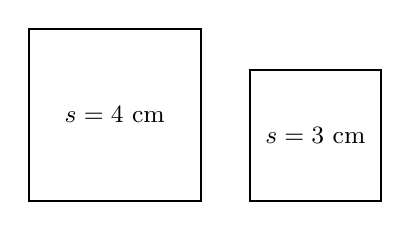
\begin{tikzpicture}[scale=0.52]
  \draw[thick] (0,0) rectangle (4.2,4.2);
  \node[font=\small] at (2.1,2.1) {$s = 4$ cm};
  \draw[thick] (5.4,0) rectangle (8.6,3.2);
  \node[font=\small] at (7.0,1.6) {$s = 3$ cm};
\end{tikzpicture}
\end{center}
\end{questionText}
\correctAnswer{$25$ cm$^2$}
\explanation{Area $1$: $4^2 = 16$ cm$^2$. Area $2$: $3^2 = 9$ cm$^2$. Total: $16 + 9 = 25$ cm$^2$.}
\end{practiceQuestion}

\begin{practiceQuestion}{3-9-q26}{gsa}
\begin{questionText}
Use the number line to estimate $\sqrt{45}$ to the nearest tenth.

\begin{center}
\begin{tikzpicture}[scale=1.05]
  \draw[thick,->] (5.5,0) -- (8.5,0);
  \foreach \x in {6,7,8} \draw (\x,0.1) -- (\x,-0.1) node[below,font=\small] {$\x$};
  \foreach \x in {6.1,6.2,...,7.9} \draw (\x,0.05) -- (\x,-0.05);
  \node[above left,font=\small] at (6.12,0.08) {$\sqrt{36}$};
  \node[above right,font=\small] at (6.88,0.08) {$\sqrt{49}$};
  \fill[funBlue] (6.7,0) circle (0.1);
  \node[above,font=\small,funBlue] at (6.7,0.38) {$\sqrt{45} \approx ?$};
\end{tikzpicture}
\end{center}
\end{questionText}
\correctAnswer{$\approx 6.7$}
\explanation{$6^2 = 36$ and $7^2 = 49$. $45$ is $\dfrac{9}{13}$ of the way from $36$ to $49$, about $0.69$. So $\sqrt{45} \approx 6.7$.}
\end{practiceQuestion}

\begin{practiceQuestion}{3-9-q27}{gsa}
\begin{questionText}
Complete the table of perfect squares.

\begin{center}
\begin{tabular}{|c|c|}
\hline
\textbf{$n$} & \textbf{$n^2$} \\
\hline
$11$ & $121$ \\ \hline
$12$ & ? \\ \hline
$13$ & $169$ \\ \hline
$14$ & ? \\ \hline
\end{tabular}
\end{center}
\end{questionText}
\correctAnswer{$12^2 = 144$ and $14^2 = 196$}
\explanation{$12 \times 12 = 144$ and $14 \times 14 = 196$.}
\end{practiceQuestion}
